%
\subsection{Обзор принципиальных схем и оборудования для сушки барды} 

На сегодняшний день принято два принципиально различных технологических процесса сушки послеспиртовой барды. 
Первый основан на методе выпаривания воды из барды и получения сухого остатка для дальнейшей переработки. 
Анализ этого процесса показывает, что энергоемкость установленного оборудования только в части электроэнергии составляет 304 кВт на установке переработки барды производительностью 300 м$^{3}$/сутки \cite{Ryabov_2003_6_Journal}. 
В зависимости от содержания сухих веществ в барде количество удаляемой влаги при сушке находится в пределах 89\dots95 кг на 100 кг барды. 
Сушка барды в натуральном виде связана с большим расходом топлива, так как на 1 кг испаряемой влаги необходимо затратить около 1 кг пара \cite{Denshikov_1963,Hug_1987_Journal}. 
Из-за сложности и высоко неоправданной стоимости проведения процесса первая схема сушки послеспиртовой барды не нашла широкое распространение в спиртовой промышленности. 
Второй процесс сушки основан на фильтрации барды, а затем окончательной сушке продукта, полученного после фильтрации. 
Отделение воды от барды возможно двумя путями: с помощью центрифугирования или с помощью различных фильтров с использованием бесконечного фильтрующего элемента \cite{Antipov_2005_2_Journal}. 
Известна типовая схема получения сухой барды, относящаяся ко второму процессу, в которой исходная барда подвергается механическому разделению фильтрацией на грубодисперсную фазу (дробину) и грубый фильтрат, содержащий взвешенные частицы, для освобождения от которых он подвергается отстаиванию в отстойнике \cite{Denshikov_1963}. 
Отстоенный фильтрат упаривается в традиционных многокорпусных установках и сушится до конечной влажности 10\% на паровой вальцовой сушилке, а дробина доводится до сухого состояния либо самостоятельно, либо в смеси с упаренным концентратом на барабанной сушилке. 
Таким образом, из барды по этой схеме можно получить два продукта: сухую барду "--- высушенную дробину с частичным добавлением фильтрата барды и экстракт барды "--- высушенные растворимые вещества барды. 
Анализ этого процесса показывает, что для его осуществления необходимо большое количество пара, что вызывает значительный расход топлива. 
К недостаткам данной схемы производства сухой барды можно также отнести следующее: использование морально устаревших сушильных аппаратов, которые при высоком потреблении энергии на сушку, не обеспечивают требуемой производительности и качества готового продукта; низкая производительность из-за применения отстойников; вследствие вязкости упаренного фильтрата выпарка требует частой механической чистки; сложность и металлоемкость производства, что обуславливает высокие эксплутационные затраты. 
Говоря о втором технологическом приеме, который получил широкое распространение, нельзя не упомянуть о современных <<гигантах>> мировой спиртовой промышленности. 
Так, на промышленном предприятии компании <<Agroetanol>> (Щвеция), которое было спроектировано и построено в 1999 г., мощностью 15~000 дал/сут топливного этанола (абсолютного спирта), используется схема обезвоживания послеспиртовой барды компании <<Alfa Laval>>, представленная на рис.~\ref{Agroetanol} принцип действия схемы в следующем. 
Послеспиртовая барда из бражной колонны (рис.~\ref{Agroetanol} ) поступает на обезвоживание, которое проводится в три стадии: на первой стадии процесс происходит в трех декантерных центрифугах <<Alfa Laval>> (рис.~\ref{Decantor}); на второй (чистая фаза) отфугованная барда концентрируется в трех пластинчатых испарителях <<Alfa Laval>> {AlfaVap) до концентрации 35\% СВ. 

\begin{figure}[h!] 
\centering 
\begin{small} 
\def\svgwidth{0.8\linewidth} 
\input{figures/Agroetanol.pdf_tex} 
\end{small} 
\caption{Схема обезвоживания послеспиртовой барды на предприятии компании <<Agroetanol>>} 
\label{Agroetanol} 
\end{figure} 

\begin{figure}[h!] 
\center{\includegraphics[width=0.8\linewidth]{Decantor.pdf}} \caption{Декантер компании <<AlfaLaval>>} 
\label{Decantor} 
\end{figure} 

Тяжёлая твёрдая фракция из декантера направляется в миксер, где смешивается с концентрированной 35\%--ной бардой. Далее данная смесь поступает в осушитель для получения сухой послеспиртовой барды (DDGS). 
Недостатками схемы <<Alfa Laval>> является то, что она использует три сложных в обслуживании пластинчатых выпарных аппарата (рис.~\ref{Plast} ) и упаривание фильтрата барды усложняется ещё тем, что в нём имеются белковые 

\begin{figure}
\centering
\begin{small} 
\def\svgwidth{1\linewidth} 
\input{figures/alfavap.pdf_tex} 
\end{small} 
\caption{Пластинчатый выпарной аппарат <<AlfaVap>>} 
\label{Plast} 
\end{figure} 

соединения и при влажности свыше 75~\% частицы сильно прилипают к паровым трубам и дальнейшее концентрирование становится затруднительной \cite{Fuks_1951}, поэтому данные аппараты часто <<засоряются>>. 
Кроме того, большая часть растворимых веществ барды, как, например, сахара, белки, при повышенной температуре легко разрушаются. 
Рассмотрим прогрессивное оборудование третьего поколения, предлагаемое компанией <<Westfalia Separator>>, для механического обезвоживания барды с получением твёрдого концентрата.
На рис.~\ref{Decan} показана конструкция декантера компании <<Westfalia Separator>> (ФРГ) на рис.~\ref{DublDec} "--- декантеры в процессе обезвоживания барды. 

\begin{figure}
\centering 
\begin{small} 
\def\svgwidth{0.8\linewidth} 
\input{figures/Westfalia.pdf_tex} 
\end{small} 
\caption{Конструкция декантера <<Westfalia Separator>> для обезвоживания барды} 
\label{Decan} 
\end{figure} 

\begin{figure}[h!] 
\center{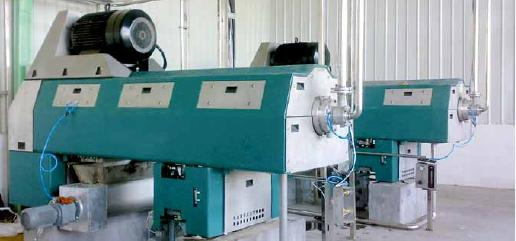
\includegraphics[width=0.8\linewidth]{WestfaliaDouble.jpeg}} 
\caption{ Два декантера <<Westfalia Sepparator>> в процессе обезвоживания барды} 
\label{DublDec} 
\end{figure} 

Основные части декантера <<Westfalia Separator>> "--- барабан и расположенный внутри барабана винтовой шнек. 
Барабан декантера вращается со скоростью в несколько тысяч оборотов в минуту, шнек барды вращается с дифференциальной скоростью, немного большей скорости вращения барабана. 
Исходная барда, поступая внутрь барабана, попадает в поле центробежных сил. 
При этом происходит разделение барды на две фазы: тяжёлую -- твёрдые частицы, которые отбрасываются к стенкам барабана, и лёгкую "--- осветленную тонкую барду, которая выделяется в центральной части барабана ближе к оси вращения. 
Выделенные твёрдые частицы транспортируются винтовым шнеком к конической части барабана (зоне сушки), где происходят их обезвоживание и выгрузка. 
Отвод тонкой барды из декантера осуществляется самотеком или при помощи напорного диска, и далее она поступает на выпарную станцию. 
Степень обезвоживания концентрата барды после сепарации составляет порядка 30\% по сухому веществу. В зависимости от количества исходной барды на стадии обезвоживания могут быть использованы декантеры различной производительности. 
Отечественными учеными Ламм Э.Л., Волчек A.M. и др \cite{Patent_2128688} предложен способ сушки суспензии послеспиртовой барды с получением кормопродукта, включающий анаэробную ферментацию путем последовательного воздействия на компоненты барды комплекса ферментов и кислотообразующих бактерий с получением культуральной жидкости и осадка белкового кормопродукта. 
Существенными недостатками предложенного способа являются: высокая стоимость осуществления из-за сложности технологического процесса; низкая производительность из-за длительности процесса; взрывоопасность; применение сложного и энергоемкого сушильного оборудования. 
Наиболее рациональным и экономически выгодным способом утилизации послеспиртовой зерновой барды является поточная линия для производства сухого белково-витаминного продукта \cite{Patent_2217490}, включающая магистрали для подвода послеспиртовой барды и отвода твердых и жидких продуктов её переработки, и связанные между собой средствами межоперационной передачи, промежуточную емкость, устройство для обезвоживания, выполненное в виде вакуумного фильтра со сходящим полотном и системой непрерывной регенерации ткани, устройство подвода-отвода горячего сухого воздуха, выполненное с возможностью взаимодействия воздуха с твердыми продуктами, вентиляционной камерой и одним циклоном, сушилку, испаритель и барометрический конденсатор с магистралью подвода воды, при этом испаритель и барометрический конденсатор расположены на магистрали подвода вакуума между вакуумным фильтром и его вакуумным насосом, магистраль отвода жидких продуктов переработки связана с испарителем и выполнена в виде затвора, включающего промежуточную емкость для жидких продуктов переработки, устройство для концентрирования фильтрата "--- сепаратор, расположенное на выходе магистрали для отвода жидких продуктов переработки, смеситель, расположенный перед гранулятором и связанный с сепаратором, гранулятор, сборник готовой продукции и устройство для упаковки. 
На сегодняшний день данная линия производства белково-витаминного продукта является одной из немногих, которые позволяют получить наиболее качественный и естественный готовый сухой продукт, с сравнительно низкими капитальными и эксплутационными затратами. 
Однако и ей присущи недостатки: в линии используется роторно-барабанная сушилка, а так как по своему составу барда является высоковлажным и полидисперсным материалам, то при сушке барды в ней наблюдается агрегатирование, комкование, налипание частиц на стенки сушильной камеры, а вследствие этого неоднородность высушивания и возможно обугливание мелких частиц продукта и инкрустация поверхности нагрева частичками барды; высокая энергоемкость процесса из-за использования предварительной сушки дробины перед сушилкой и большого количества вентиляторов; высокая степень уноса частиц продукта, а вследствие этого использование в линии дополнительных циклонов; неэффективное применение сепаратора для концентрирования фильтрата; линия не предусматривает более полное использование компонентов послеспиртовой барды и очистку жидкого отхода, так как не указывается дальнейшее предназначение сепарированного фильтрата. 
В настоящее время в нашей стране машиностроительная промышленность только с недавнего времени начала разрабатывать и внедрять в производство сушильные аппараты для сушки послеспиртовой барды. 
Так, ОАО <<Нежинский механиический завод>> выпускает контактные роторно-дисковые сушилки типа СКМ, (рис.~\ref{CKM} ) 
Корпус представляет собой стальной цилиндр, имеюший паровую рубашку, загрузочный и разгрузочный люк с шибером. 

\begin{figure} 
\centering 
\begin{footnotesize} 
\def\svgwidth{0.95\linewidth} 
\input{figures/DDGS.pdf_tex} 
\end{footnotesize} 
\caption{Сушилка СКМ Нежинского механического завода} 
\label{CKM} 
\end{figure} 

Последний предназначен для регулировки уровня продукта в сушилке. 
Для полного опорожнения сушилки от барды имеется окно. 
Вал представляет собой трубу с расположенными на нём полыми дисками. 
На дисках закреплены лопатки для перемешивания барды и перемещения её к разгрузочному люку. Между дисками устанавливаются скребки для предотвращения застревания продукта и его рыхления. 
Сушка предварительно сгущенной барды происходит за счёт соприкосновения барды с нагреваемыми паром поверхностями дисков, корпуса и вала. 
Кроме того, барда, продвигаясь в осевом направлении, дополнительно сушится встречным потоком воздуха. 
В целях полного использования греющих поверхностей сушилка должна заполняться высушиваемым продуктом на 2/3 объёма корпуса, что контролируется через смотровые окна на боковой крышке. 
Скорость продвижения материала в сушилке можно регулировать изменением положения лопаток во встречных направлениях.
 Аналогичные контактные сушилки марки TST выпускает норвежская фирма <<Stord Internaional>>, а марки PGI-300B -- Цзилинский завод сушильных агрегатов (Китай). 
Конструктивно похожие контактные сушилки шнекового типа марки 133.4 и 133.7 производит ОАО <<Уралхиммаш>> \cite{Korman_2003_7_Journal}. 
Однако процесс сушки послеспиртовой барды в данных аппаратах сопровождается с определенными сложностями. 
Так как при снижении влажности в барде проявляются хорошо выраженные адгезионные и когезионные свойства, барда приобретает студенистую консистенцию, все более густую и при перемешивании наблюдается окомкование (указанные факторы затрудняют процесс обезвоживания), а также данные установки обладают высокой материалоемкостью и энергоемкостью (потребление пара, кг на кг испаренной влаги "--- 1,47). 
Подводя итог вышесказанному, можно сделать вывод, что на данный момент в нашей стране, Европе, США и других странах существует проблема в утилизации послеспиртовой зерновой барде, в несовершенстве технологий и технологического оборудования для осуществления процесса сушки барды. 
Проведя литературный обзор и патентный поиск, выяснилось, что сушку барды в России, Европе, США и ряде других стран проводят преимущественно в барабанных, ленточных, слоевых и ротационных сушилках, которые при высоком потреблении энергии на сушку, не обеспечивают требуемой производительности и качества готового продукта \cite{Antipov_2005_2_Journal,Zhuravlev_2004}. 
Поэтому необходимо совершенствование процесса сушки послеспиртовой барды и оборудования для его осуществления. 
В результате проведения аналитического исследования выявилось, что, так как барда является полидисперсным материалом (неоднородным по составу), то при сушке барды наблюдается комкование, неоднородность высушивания, налипание частиц на стенки сушилки, обугливание мелких частиц продукта и инкрустация поверхности нагрева частичками барды. 
Анализ выявленных особенностей показал целесообразность использования такого вида сушки, при котором каждая частица барды получала бы необходимое количество энергии для фазового превращения содержащейся в ней влаги без образования крупных соединений частиц.